\section{Auswertung}
\label{sec:Auswertung}

\subsection{Überprüfung der Stabilitätsbedingung}

\begin{figure}
    \centering
    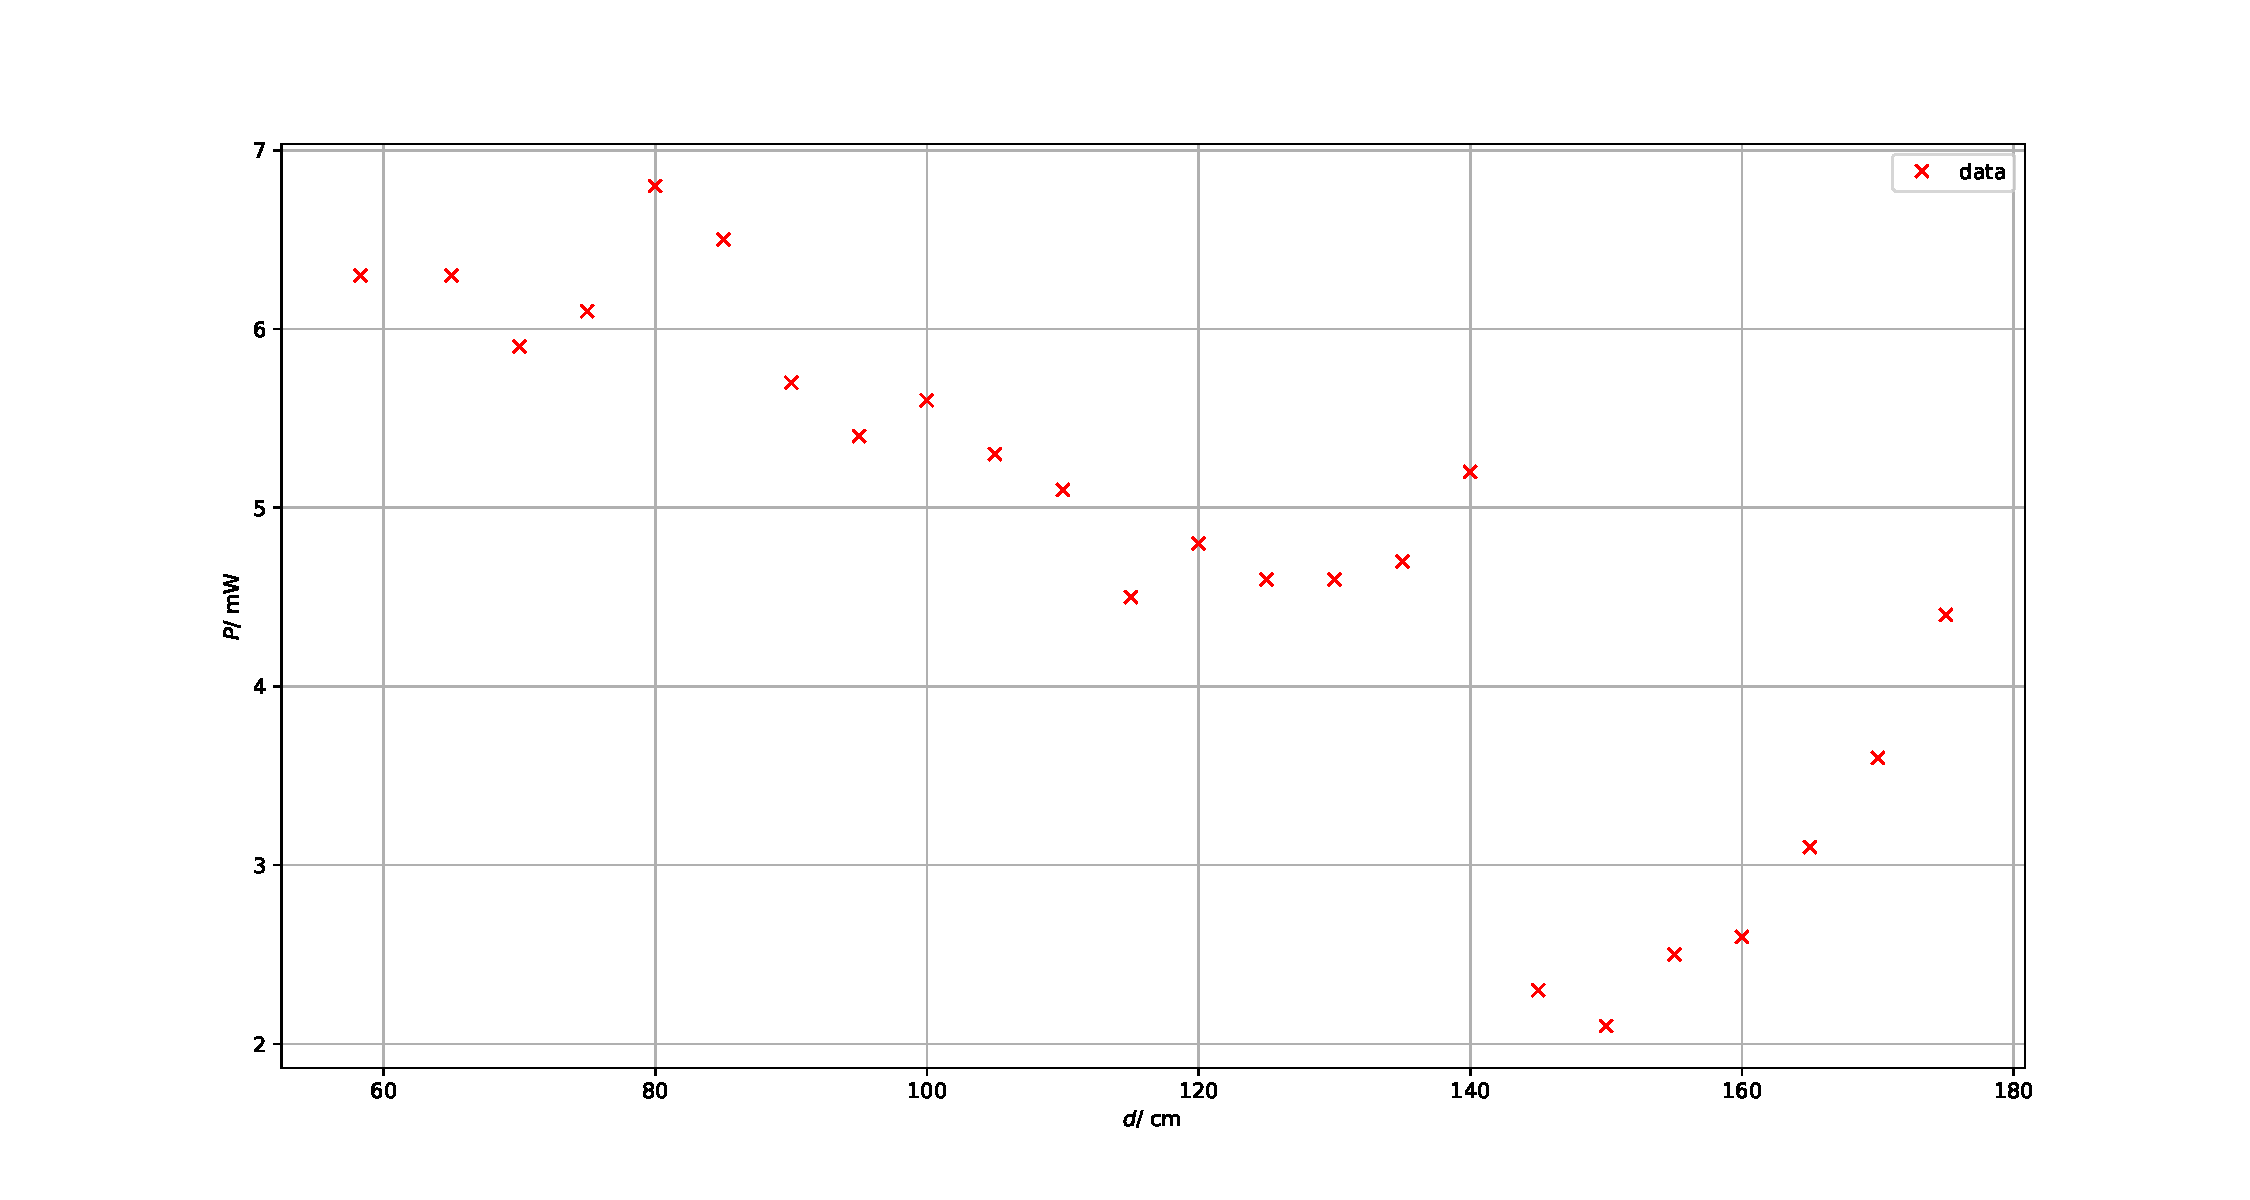
\includegraphics[width=12cm]{plots/stability140.pdf}
    \caption{Die Resonatorlänge ist gegen die Leistung aufgetragen. Dabei besteht der Resonator aus zwei konkaven Spiegeln mit jeweils $b_\text{i} = \SI{140}{\centi\meter}$.}
    \label{fig:stability140}
\end{figure}   

\begin{figure}
    \centering
    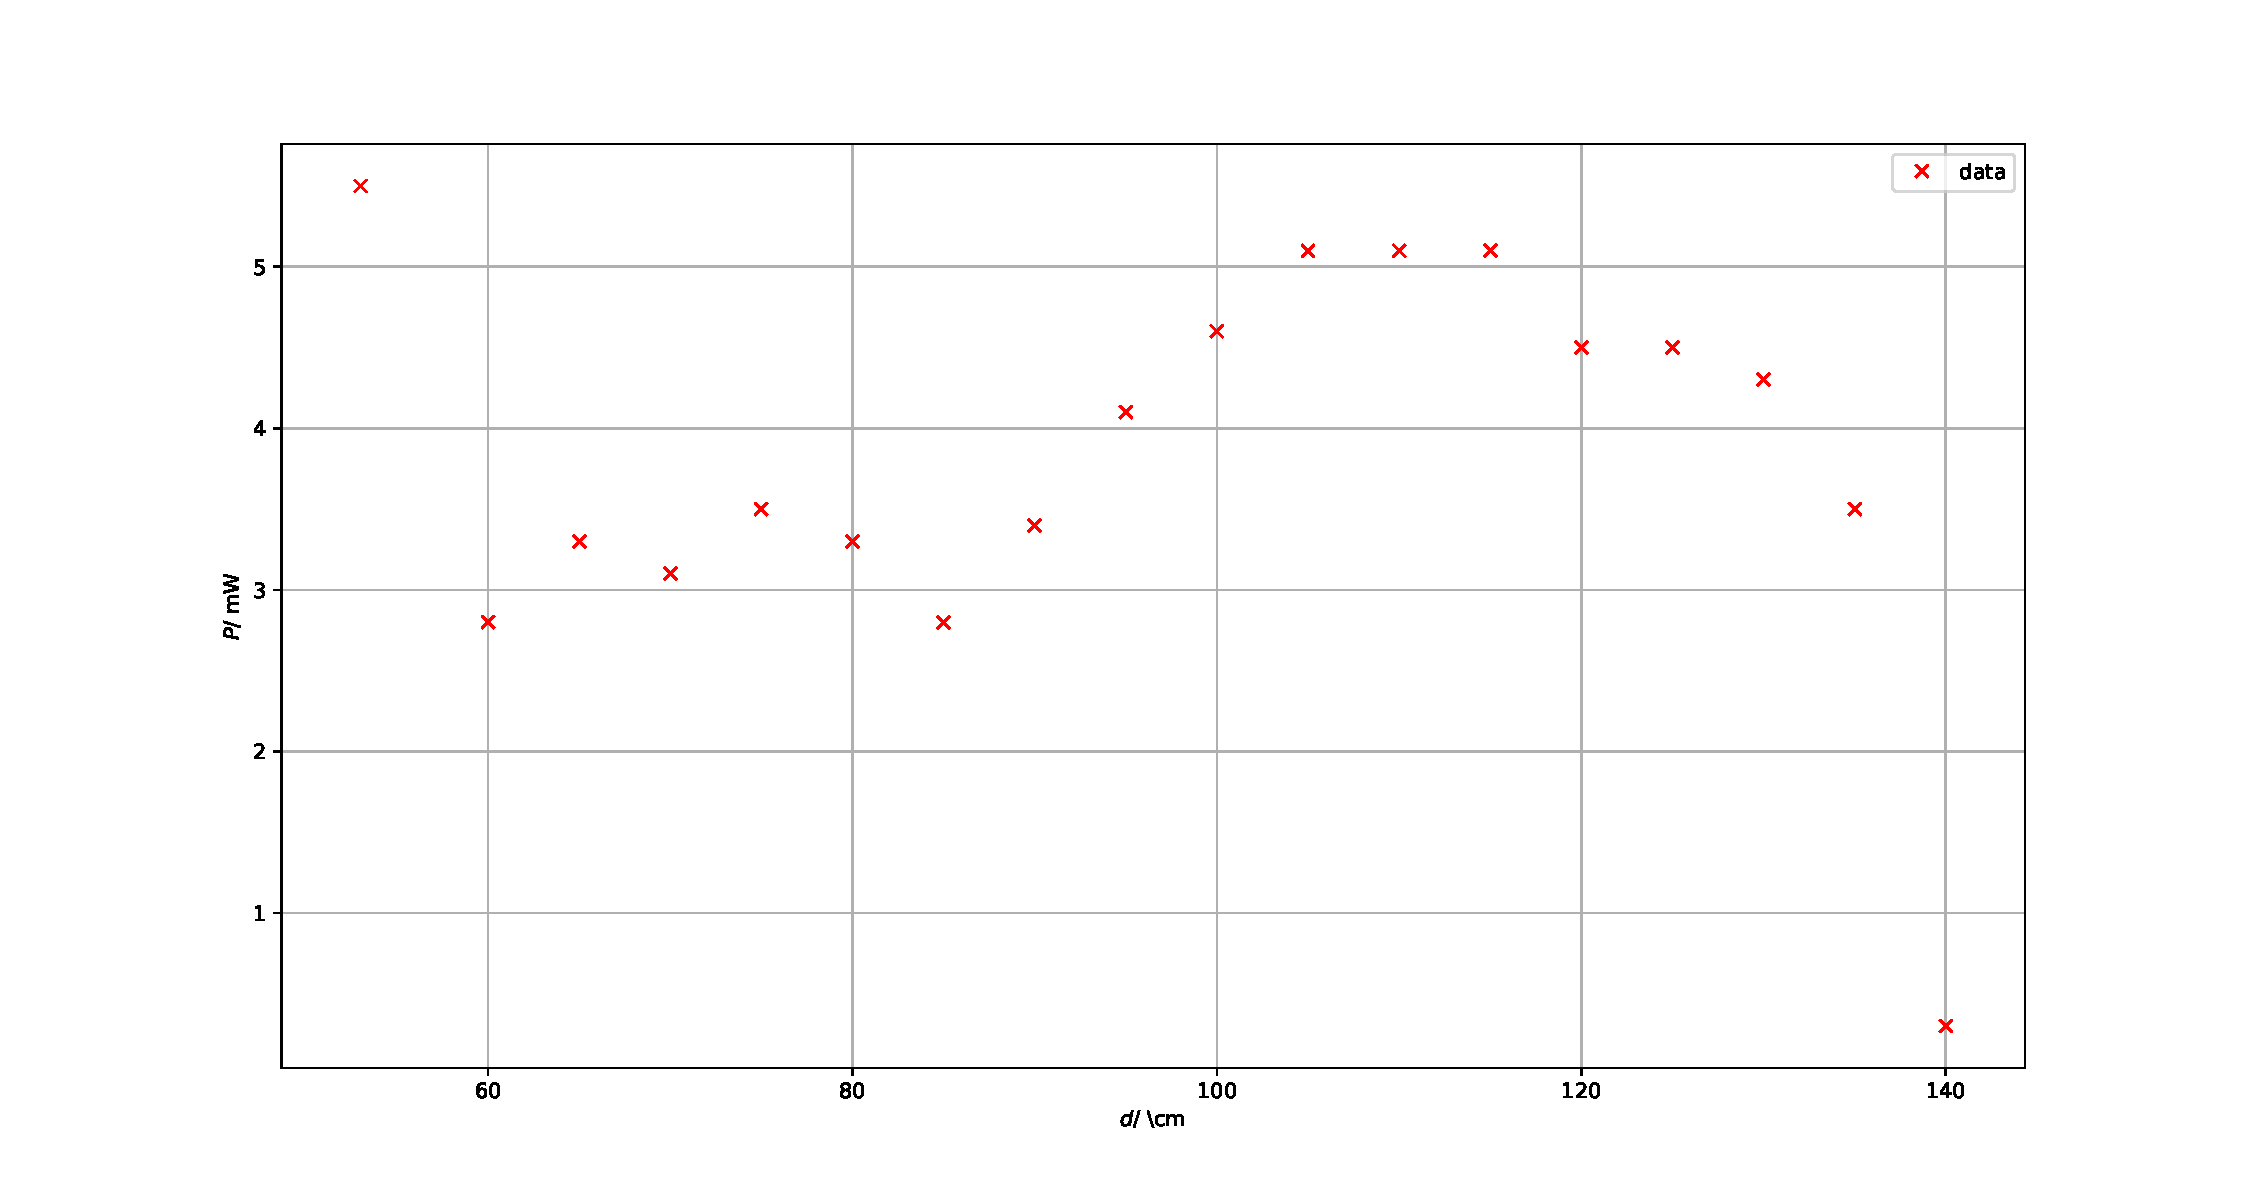
\includegraphics[width=12cm]{plots/stability_flat.pdf}
    \caption{Die Resonatorlänge ist gegen die Leistung aufgetragen. Dabei besteht der Resonator aus einem flachen und einem konkaven Spiegel mit $b_2 = \SI{140}{\centi\meter}$.}
    \label{fig:stability_flat}
\end{figure} 

\subsection{Vermessung von TEM-Moden}

\begin{figure}
    \centering
    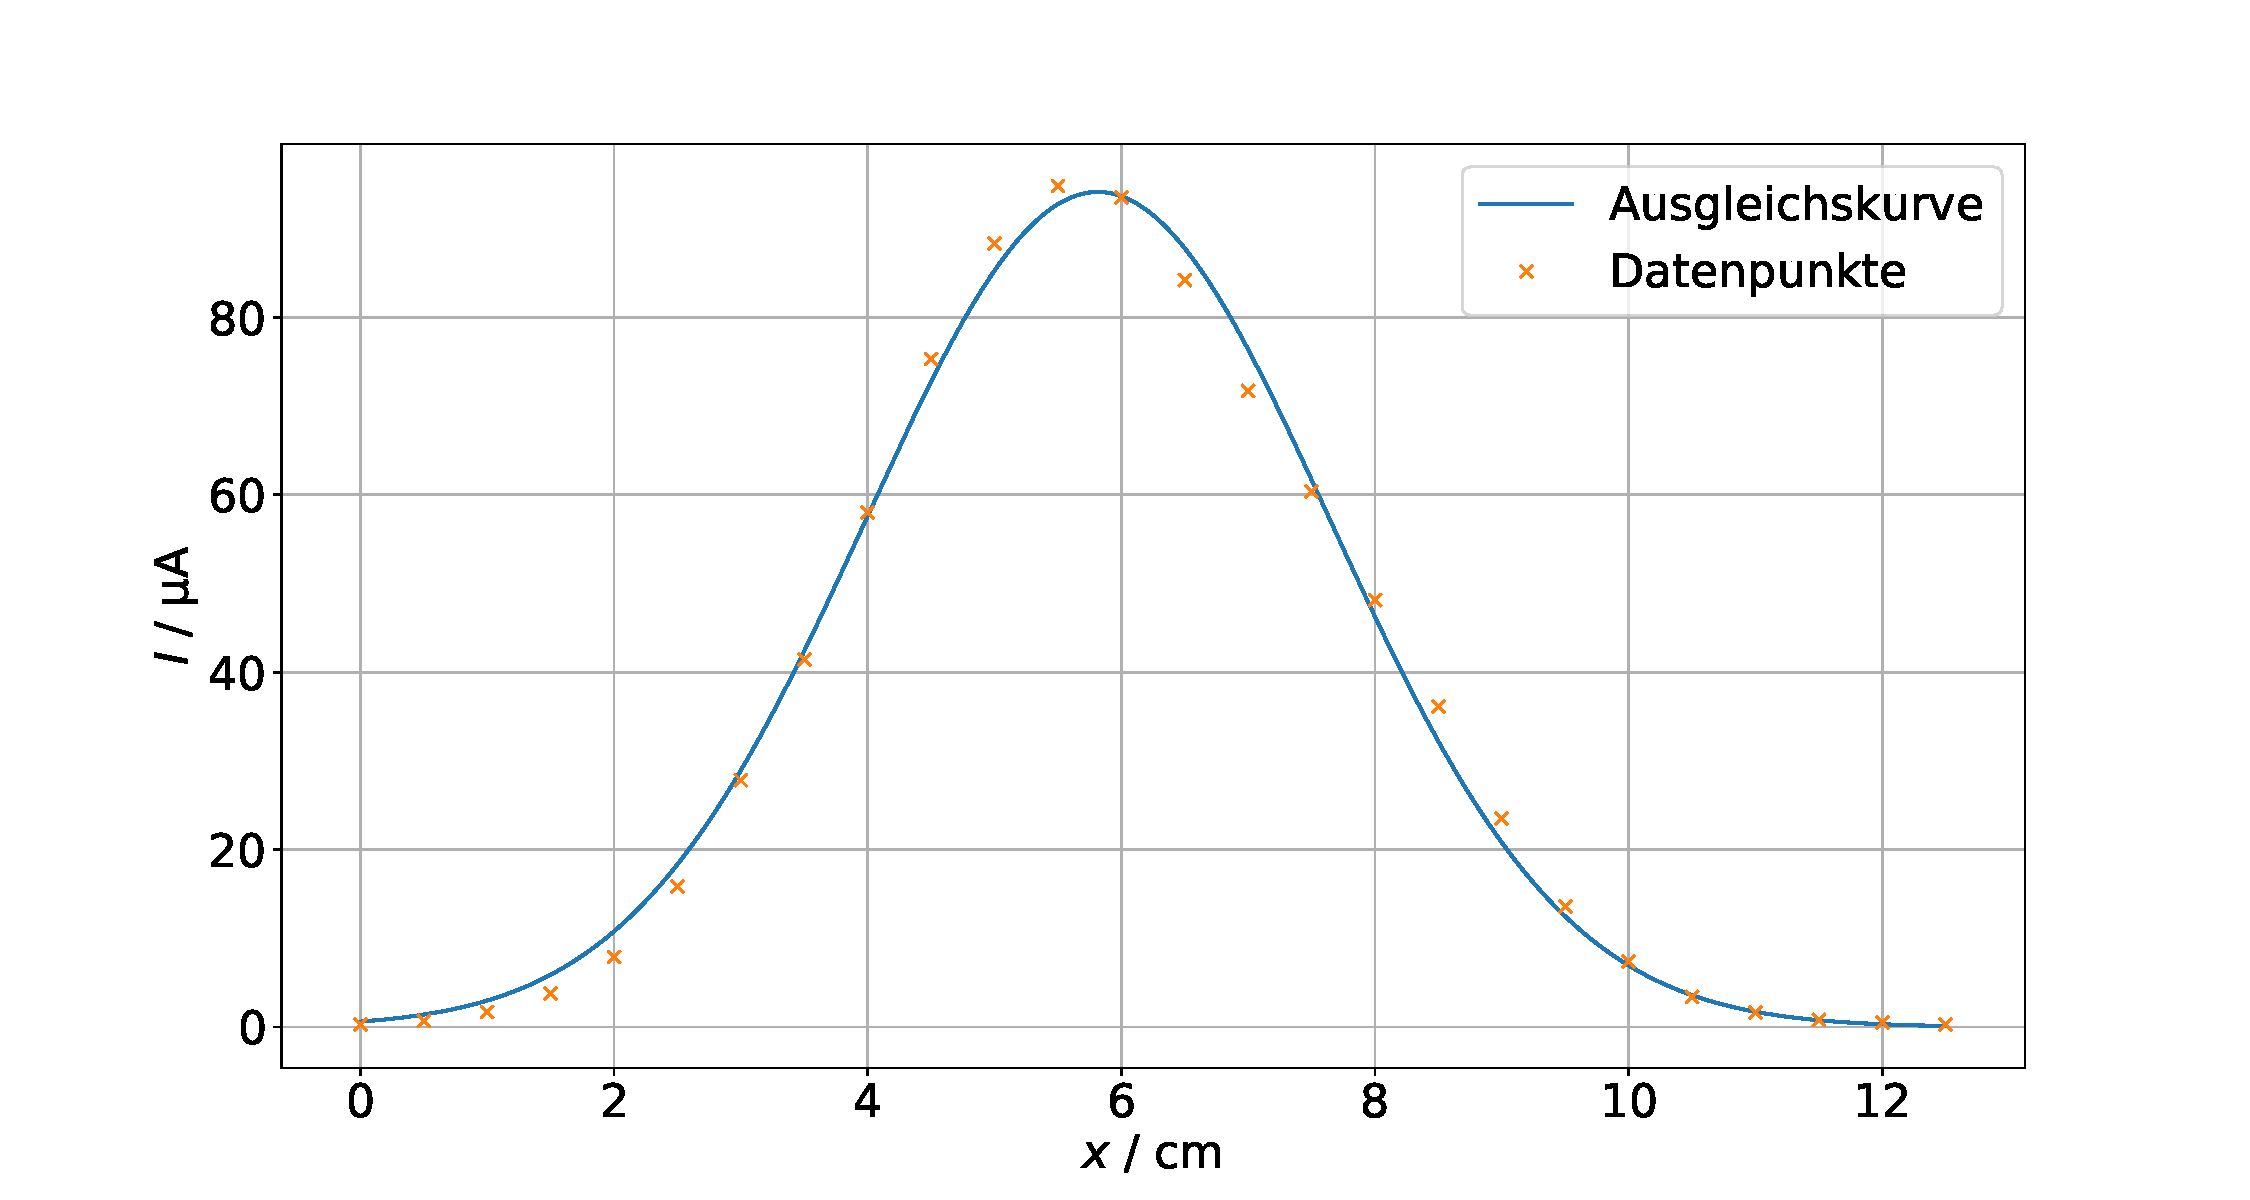
\includegraphics[width=12cm]{plots/mode0.pdf}
    \caption{Der Abstand senkrecht zur Laserachse ist gegen die gemessene Stromstärke aufgetragen. Zu sehen ist die TEM$_{00}-$Mode.}
    \label{fig:mode0}
\end{figure}

\begin{figure}
    \centering
    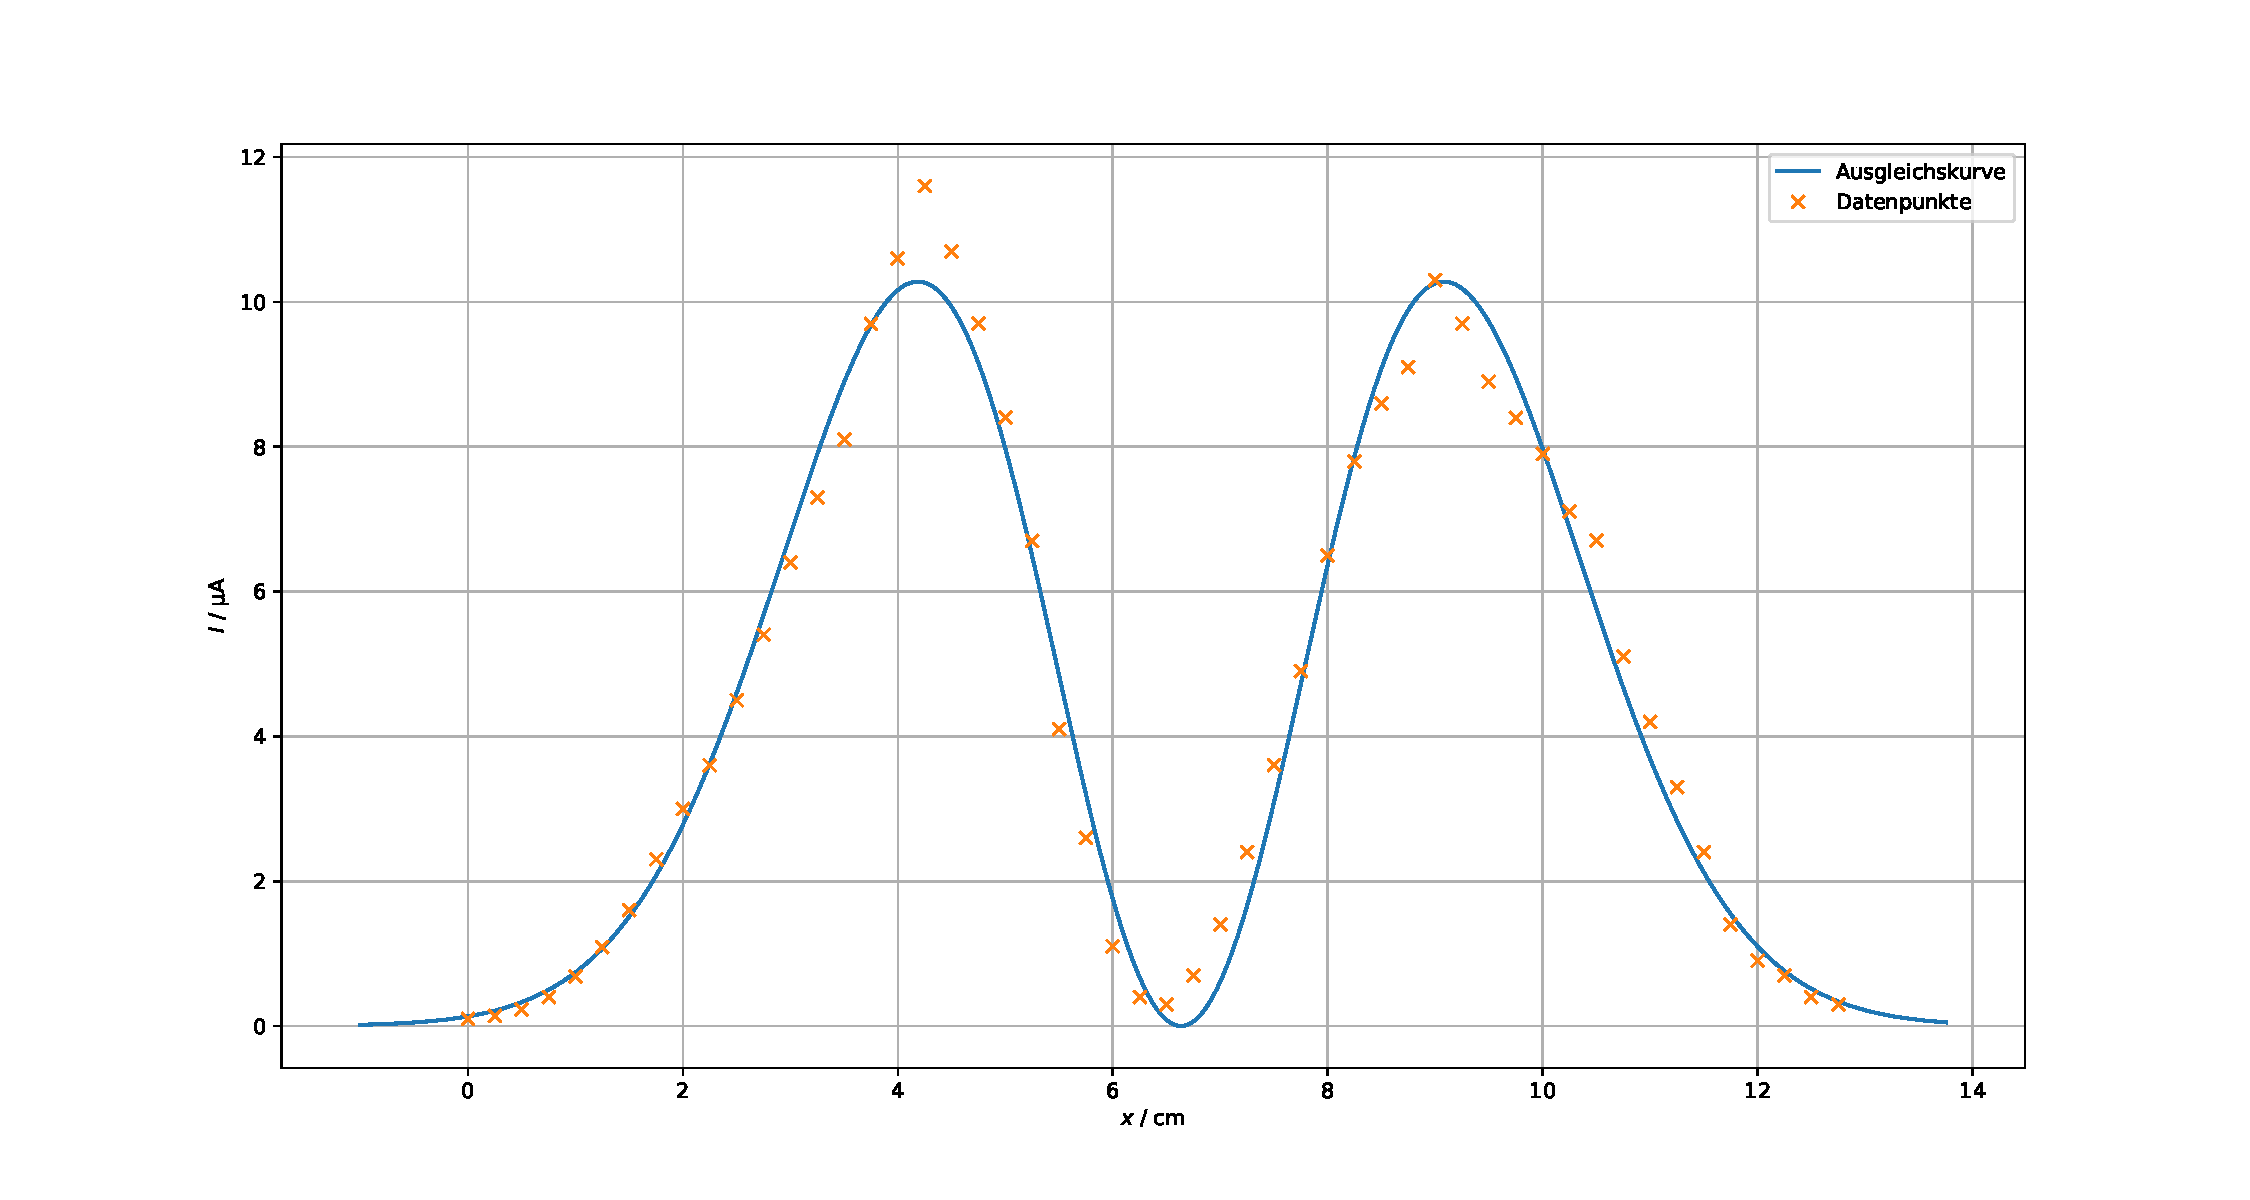
\includegraphics[width=12cm]{plots/mode1.pdf}
    \caption{Der Abstand senkrecht zur Laserachse ist gegen die gemessene Stromstärke aufgetragen. Zu sehen ist die TEM$_{01}-$Mode.}
    \label{fig:mode1}
\end{figure}

\begin{figure}
    \centering
    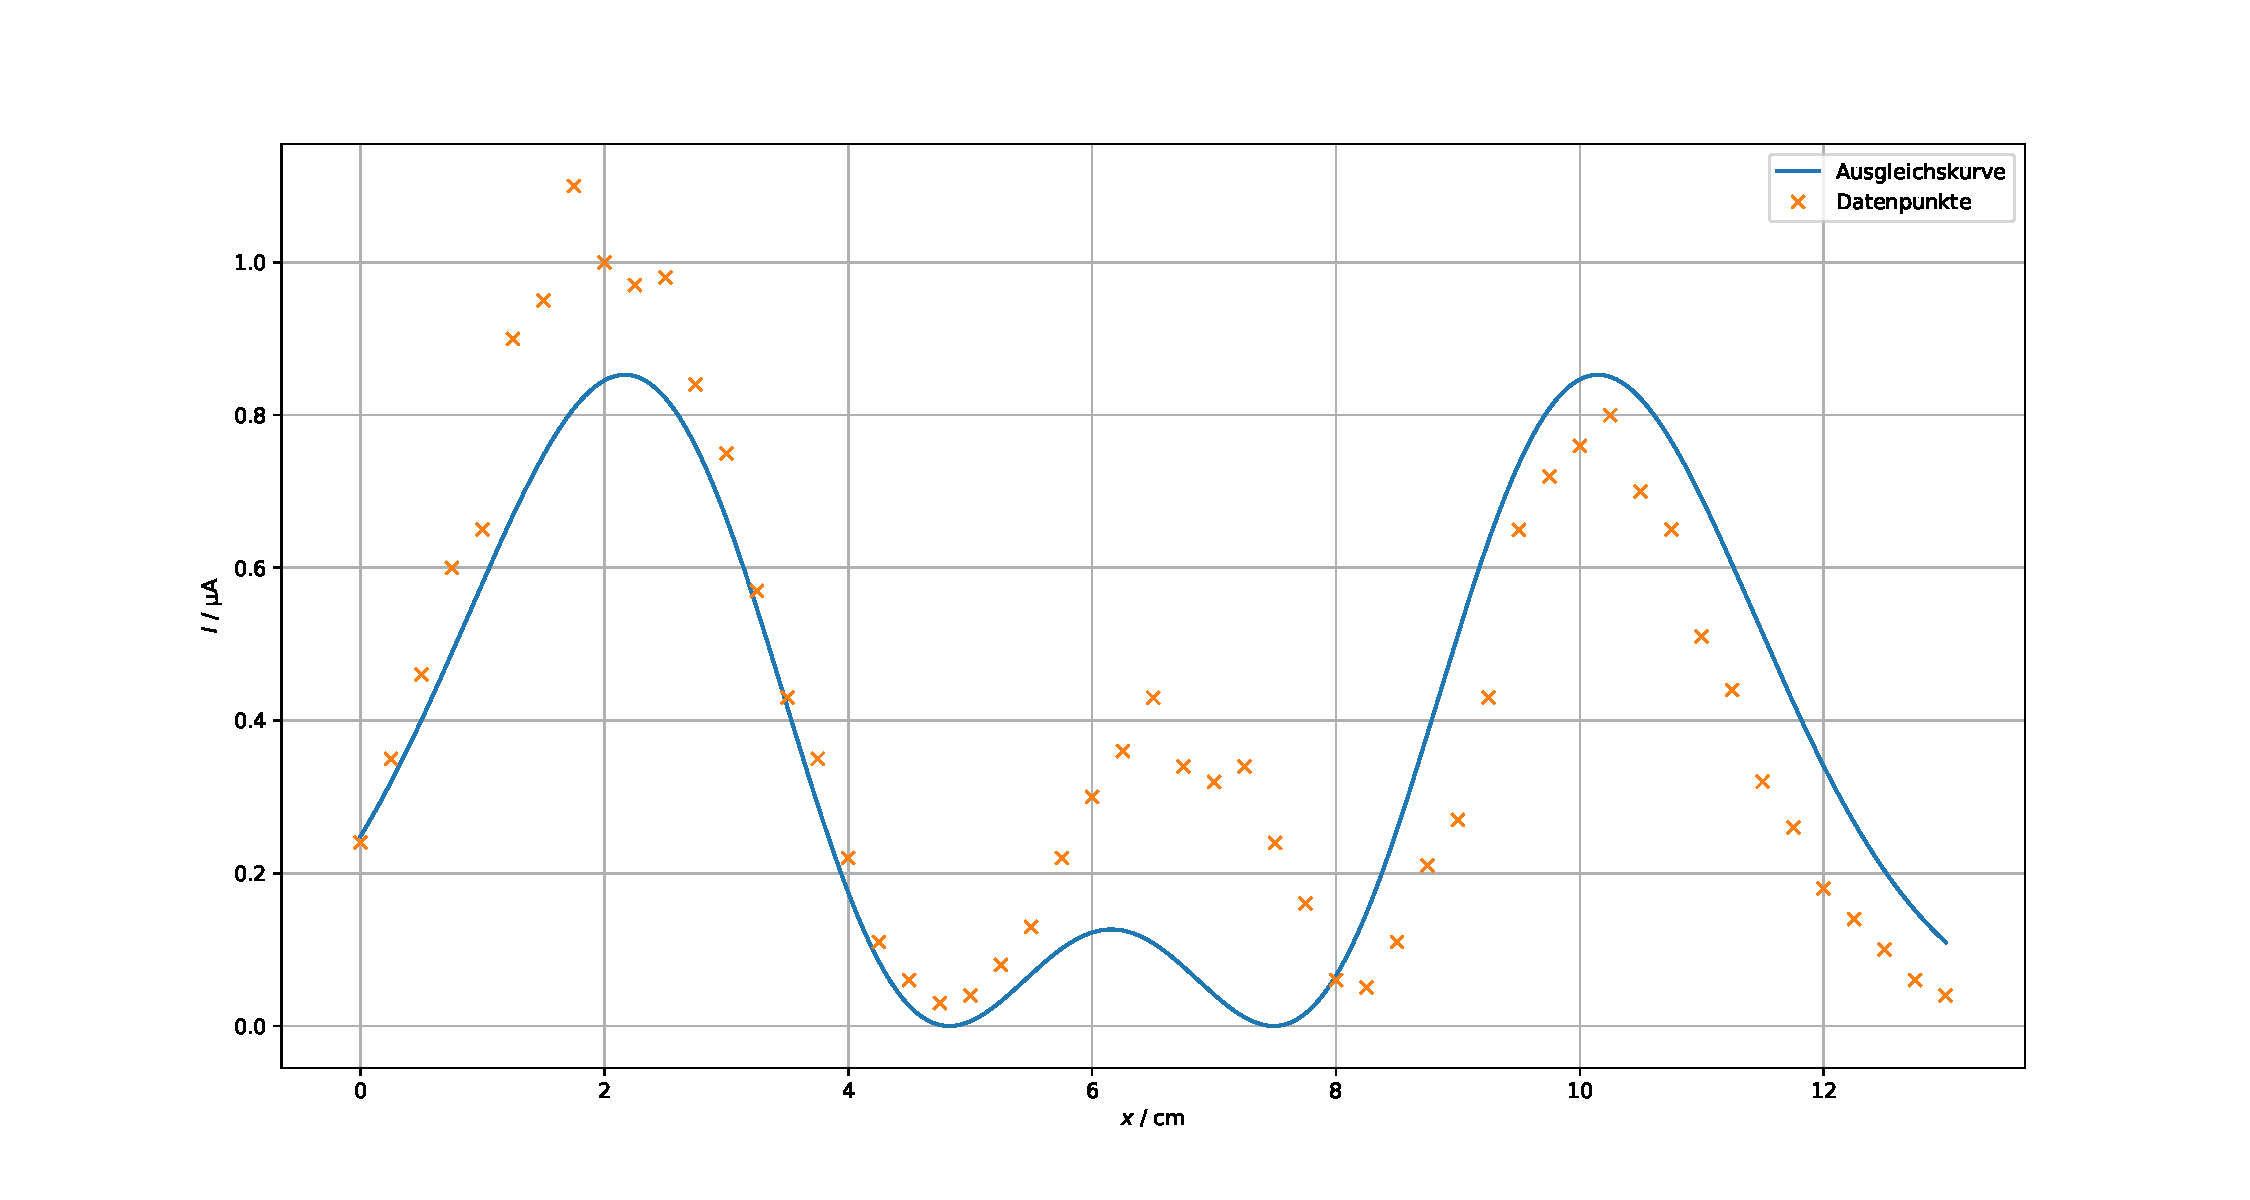
\includegraphics[width=12cm]{plots/mode2.pdf}
    \caption{Der Abstand senkrecht zur Laserachse ist gegen die gemessene Stromstärke aufgetragen. Zu sehen ist die TEM$_{02}-$Mode.}
    \label{fig:mode2}
\end{figure}

\subsection{Messung der Polarisation}

\begin{figure}
    \centering
    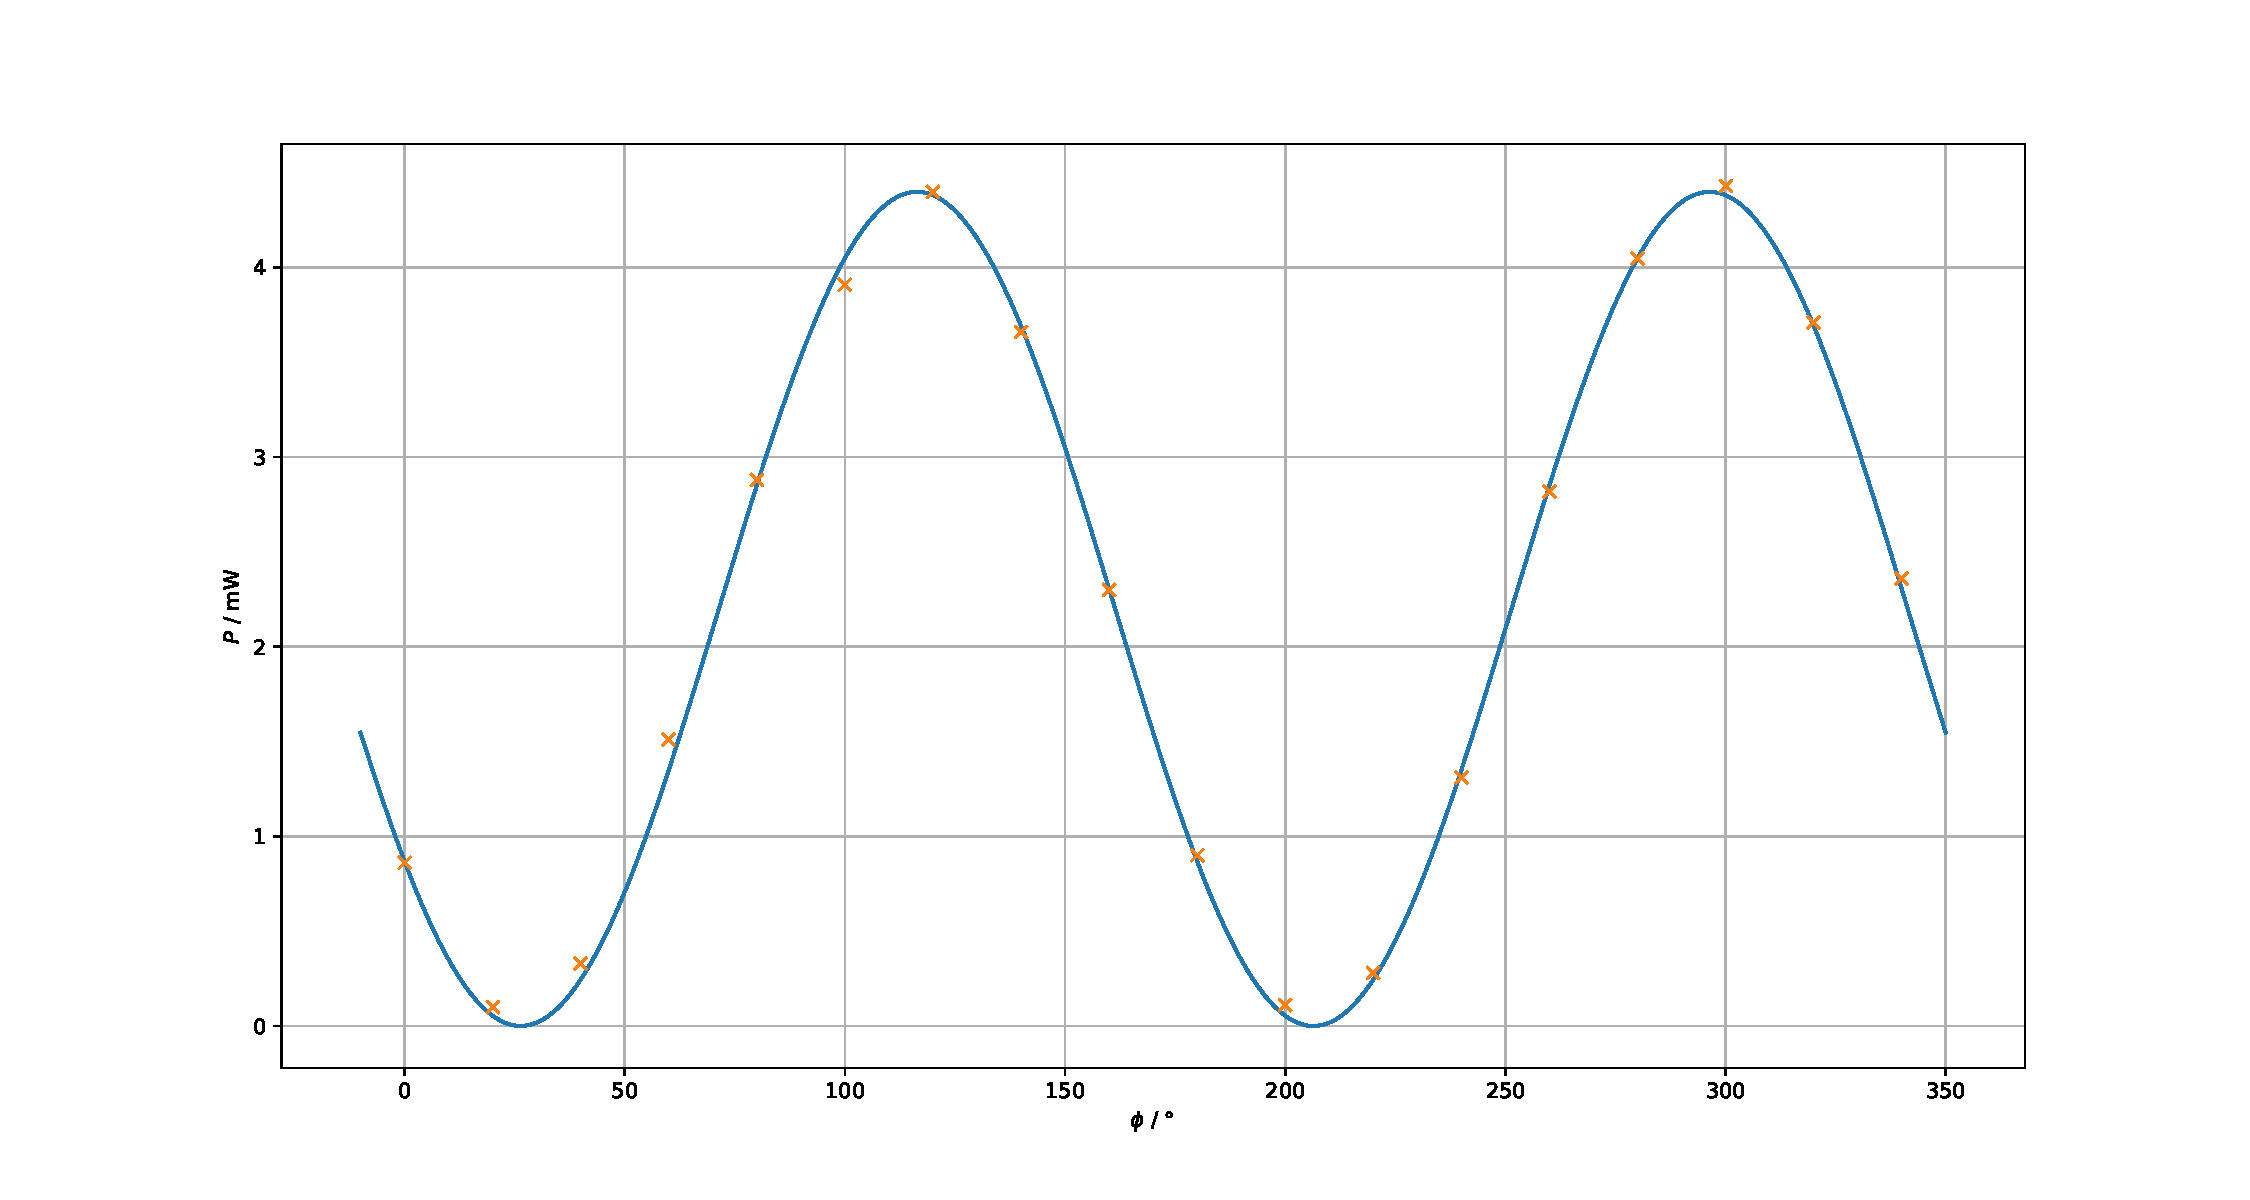
\includegraphics[width=12cm]{plots/polarisation.pdf}
    \caption{Der Polarisationswinkel ist gegen die Leistung aufgetragen.}
    \label{fig:polarisation}
\end{figure}    

\subsection{Bestimmung der Wellenlänge}

